% ============================================================
% body.tex —— 答案册一页样页内容（demo 自拟题例，非题库题）
% 演示覆盖项（任务书要求各一）：分区标题行／题号＋答案行／解析两栏／带图解答例／多行答案例。
% 题例自拟、逐题亲算（数值已手工复核），仅作式样演示，不入题池、不承内容守恒。
% ============================================================
\zhangtitle{第一章\quad 空间向量与立体几何}
\jietitle{1.1.1\quad 空间向量及其运算(练习件答案)}

\begin{multicols}{2}
\raggedcolumns
\emergencystretch=1em

\qufen{一、选择题}{本组共2题}

\ansitem{1}{A}
\ansline{分析}{把\(|\overrightarrow{a} + \overrightarrow{b}|\)先用数量积展开，再代入已知的模与数量积即可．}
\ansline{详解}{\(|\overrightarrow{a} + \overrightarrow{b}|^{2} = |\overrightarrow{a}|^{2} + 2\overrightarrow{a} \cdot \overrightarrow{b} + |\overrightarrow{b}|^{2} = 4 + 2 \times ( - 3) + 9 = 7\)，所以\(|\overrightarrow{a} + \overrightarrow{b}| = \sqrt{7}\)．故选：A．}

\ansitem{2}{C}
\ansline{分析}{由数量积的定义式反解夹角余弦，再在\(0^{\circ}\)到\(180^{\circ}\)内定角．}
\ansline{详解}{由\(\overrightarrow{a} \cdot \overrightarrow{b} = |\overrightarrow{a}||\overrightarrow{b}|\cos\langle \overrightarrow{a},\overrightarrow{b} \rangle\)得\(\cos\langle \overrightarrow{a},\overrightarrow{b} \rangle = \frac{- 6}{3 \times 4} = - \frac{1}{2}\)．因为\(\langle \overrightarrow{a},\overrightarrow{b} \rangle \in \lbrack 0^{\circ},180^{\circ}\rbrack\)，所以\(\langle \overrightarrow{a},\overrightarrow{b} \rangle = 120^{\circ}\)．故选：C．}

\qufen{二、填空题}{本组共2题}

\ansitem{3}{\(- 4\)}
\ansline{分析}{两向量共线即存在唯一实数\(\lambda\)使\(\overrightarrow{c} = \lambda\overrightarrow{d}\)，比较基底系数得方程组．}
\ansline{详解}{因为\(\overrightarrow{a}\)，\(\overrightarrow{b}\)不共线，故\(\overrightarrow{c}\parallel\overrightarrow{d}\)等价于存在实数\(\lambda\)使\(2\overrightarrow{a} - 3\overrightarrow{b} = \lambda(k\overrightarrow{a} + 6\overrightarrow{b}) = \lambda k\overrightarrow{a} + 6\lambda\overrightarrow{b}\)．对应系数相等，得\(2 = \lambda k\)且\(- 3 = 6\lambda\)，解得\(\lambda = - \frac{1}{2}\)，\(k = - 4\)．}

\ansitem{4}{(1)\(2\sqrt{3}\)；(2)\(4\)}
\ansline{分析}{以同一顶点出发的三条棱向量为基底，把目标向量写成基底的和，再用两两垂直消去交叉项．}
\ansline{详解}{由正方体知\(\overrightarrow{AB}\)，\(\overrightarrow{AD}\)，\(\overrightarrow{AA_{1}}\)两两垂直且模均为\(2\)．(1)\(\overrightarrow{AC_{1}} = \overrightarrow{a} + \overrightarrow{b} + \overrightarrow{c}\)，则\(|\overrightarrow{AC_{1}}|^{2} = |\overrightarrow{a}|^{2} + |\overrightarrow{b}|^{2} + |\overrightarrow{c}|^{2} + 2(\overrightarrow{a} \cdot \overrightarrow{b} + \overrightarrow{a} \cdot \overrightarrow{c} + \overrightarrow{b} \cdot \overrightarrow{c}) = 12 + 0 = 12\)，故\(AC_{1} = 2\sqrt{3}\)．(2)\(\overrightarrow{AB} \cdot \overrightarrow{AC_{1}} = \overrightarrow{a} \cdot (\overrightarrow{a} + \overrightarrow{b} + \overrightarrow{c}) = |\overrightarrow{a}|^{2} + \overrightarrow{a} \cdot \overrightarrow{b} + \overrightarrow{a} \cdot \overrightarrow{c} = 4\)．}

\qufen{三、解答题}{本组共4题}

\ansitem{5}{\(- 1\)}
\ansline{分析}{把\(\overrightarrow{AE}\)与\(\overrightarrow{BD}\)都用从\(A\)出发的三条棱向量表示，再用垂直关系与模长作数量积．}
\ansline{详解}{如图，设\(\overrightarrow{AB} = \overrightarrow{a}\)，\(\overrightarrow{AD} = \overrightarrow{b}\)，\(\overrightarrow{AA_{1}} = \overrightarrow{c}\)，则\(|\overrightarrow{a}| = |\overrightarrow{b}| = |\overrightarrow{c}| = 1\)且两两垂直．因为\(E\)为\(BB_{1}\)的中点，所以\(\overrightarrow{AE} = \overrightarrow{AB} + \overrightarrow{BE} = \overrightarrow{a} + \frac{1}{2}\overrightarrow{c}\)；又\(\overrightarrow{BD} = \overrightarrow{AD} - \overrightarrow{AB} = \overrightarrow{b} - \overrightarrow{a}\)．于是
\(\overrightarrow{AE} \cdot \overrightarrow{BD} = \allowbreak\left( \overrightarrow{a} + \frac{1}{2}\overrightarrow{c} \right) \cdot \allowbreak\left( \overrightarrow{b} - \overrightarrow{a} \right) = \overrightarrow{a} \cdot \overrightarrow{b} - |\overrightarrow{a}|^{2} + \frac{1}{2}\overrightarrow{c} \cdot \overrightarrow{b} - \frac{1}{2}\overrightarrow{c} \cdot \overrightarrow{a} = 0 - 1 + 0 - 0 = - 1\)．}
\ansfig{%
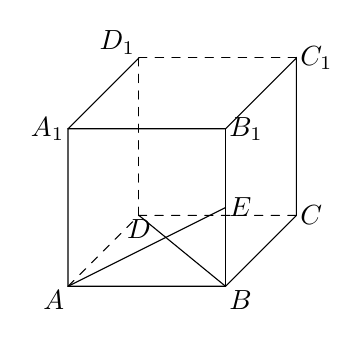
\begin{tikzpicture}[scale=1.0,line width=0.4pt,line cap=round,
    every node/.style={inner sep=1.2pt,font=\figfont}]
  \coordinate (A) at (0,0);      \coordinate (B) at (2,0);
  \coordinate (C) at (2.9,0.9);  \coordinate (D) at (0.9,0.9);
  \coordinate (A1) at (0,2);     \coordinate (B1) at (2,2);
  \coordinate (C1) at (2.9,2.9); \coordinate (D1) at (0.9,2.9);
  \coordinate (E) at (2,1);
  \draw[dashed] (A)--(D)--(C);
  \draw[dashed] (D)--(D1);
  \draw[dashed] (C1)--(D1);
  \draw (A)--(B)--(C)--(C1)--(B1)--(A1)--cycle;
  \draw (B)--(B1);
  \draw (A1)--(D1);
  \draw (A)--(E);
  \draw (B)--(D);
  \node[below left]  at (A)  {\(A\)};
  \node[below right] at (B)  {\(B\)};
  \node[right]       at (C)  {\(C\)};
  \node[below]       at (D)  {\(D\)};
  \node[left]        at (A1) {\(A_{1}\)};
  \node[right]       at (B1) {\(B_{1}\)};
  \node[right]       at (C1) {\(C_{1}\)};
  \node[above left]  at (D1) {\(D_{1}\)};
  \node[right]       at (E)  {\(E\)};
\end{tikzpicture}}

\ansitem{6}{\(- \frac{1}{4}\overrightarrow{b}\)}
\ansline{分析}{先用夹角余弦求数量积，再按投影向量公式直接代入，不必另求单位向量与夹角．}
\ansline{详解}{\(\overrightarrow{a} \cdot \overrightarrow{b} = |\overrightarrow{a}||\overrightarrow{b}|\cos 120^{\circ} = 1 \times 2 \times \left( - \frac{1}{2} \right) = - 1\)，故\(\overrightarrow{a}\)在\(\overrightarrow{b}\)上的投影向量为\(\frac{\overrightarrow{a} \cdot \overrightarrow{b}}{|\overrightarrow{b}|^{2}}\overrightarrow{b} = - \frac{1}{4}\overrightarrow{b}\)．}
\ansline{点睛}{投影向量是向量、投影数量是实数，两者名称与属性都不同，答题时不可混用．}

\ansitem{7}{\(60^{\circ}\)}
\ansline{分析}{异面直线所成角不超过\(90^{\circ}\)，先把两条直线对应的向量用基底表示，再用数量积求向量夹角。}
\ansline{详解}{设\(\overrightarrow{AB} = \overrightarrow{a}\)，\(\overrightarrow{AD} = \overrightarrow{b}\)，\(\overrightarrow{AA_{1}} = \overrightarrow{c}\)，则\(|\overrightarrow{a}| = |\overrightarrow{b}| = |\overrightarrow{c}| = 1\)且两两垂直．\(\overrightarrow{A_{1}B} = \overrightarrow{a} - \overrightarrow{c}\)，\(\overrightarrow{BC_{1}} = \overrightarrow{b} + \overrightarrow{c}\)，于是\(\overrightarrow{A_{1}B} \cdot \overrightarrow{BC_{1}} = \allowbreak\left( \overrightarrow{a} - \overrightarrow{c} \right) \cdot \allowbreak\left( \overrightarrow{b} + \overrightarrow{c} \right) = - |\overrightarrow{c}|^{2} = - 1\)；又\(|\overrightarrow{A_{1}B}| = |\overrightarrow{BC_{1}}| = \sqrt{2}\)，故\(\cos\langle \overrightarrow{A_{1}B},\overrightarrow{BC_{1}} \rangle = - \frac{1}{2}\)，向量夹角为\(120^{\circ}\)．因为异面直线所成角取\(90^{\circ}\)以内的角，所以\(A_{1}B\)与\(BC_{1}\)所成的角为\(60^{\circ}\)．}

\ansitem{8}{\(\sqrt{14}\)}
\ansline{分析}{两两垂直即两两数量积为\(0\)，把模的平方按数量积展开后交叉项全消。}
\ansline{详解}{因为\(\overrightarrow{a}\)，\(\overrightarrow{b}\)，\(\overrightarrow{c}\)两两垂直，所以\(\overrightarrow{a} \cdot \overrightarrow{b} = \overrightarrow{a} \cdot \overrightarrow{c} = \overrightarrow{b} \cdot \overrightarrow{c} = 0\)．于是\(|\overrightarrow{a} + \overrightarrow{b} + \overrightarrow{c}|^{2} = |\overrightarrow{a}|^{2} + |\overrightarrow{b}|^{2} + |\overrightarrow{c}|^{2} = 1 + 4 + 9 = 14\)，故\(|\overrightarrow{a} + \overrightarrow{b} + \overrightarrow{c}| = \sqrt{14}\)．}

\end{multicols}
